\section{Coordinate Systems: 3D}
The 3D coordinate system is defined by 8 "areas". These are called octants, which are defined by the coordinate system planes (I.E octant 1 is defined to be postive x, positive y, and positve z). 

\subsection{Equations and input space}
Equations in $\mathbb{R}^3$ should be seen as $2D$ inputs with $1D$ output. Back in graphs of $\mathbb{R}^2$, we had an $x$-axis and $y$-axis, the former being the input space and the latter being the output. In $\mathbb{R}^3$ the equations and formulas should be seen as taking $(x, y)$ points, which are ($\mathbb{R}^2$) inputs, and outputing to a single value. This mean that scaler functions of $\mathbb{R}^n$, where $n-1$ is the number of variables that function wil be. 

\section{Coordinate Systems: Lines and Planes}
\subsection{Lines}
Lines in $\mathbb{R}^3$ requires a initial position vector and some sort of "slope" vector that multipled by a scaler parameter. 

\begin{equation*}
	\vec{r_f} = \vec{r_i} + \vec{v}t 
\end{equation*}

%-------------------------------------------------------------------------%
\begin{figure}[H]
	\begin{center}
		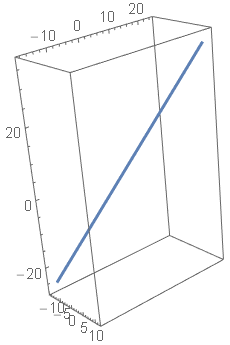
\includegraphics[scale=0.45]{pages/images/simple_line.png}
		\caption{Example of $\mathbb{R}^3$ Line}	
		\label{fig:test_figure}
	\end{center}
\end{figure}
%-------------------------------------------------------------------------%

\subsubsection{Parametric Equation of Lines}
Now the slope vector gives some sort of orientation to the line. When we think of the vector equation of a line, we can think of their components. We can think of the multiple components in the $\vec{v}$ as slopes alongside those respective axis. This way we can formulate parametric equations when considering that vectors will have $\mathbb{R}^3$ components. 
\begin{align*}
	x &= r_{ox}+v_xt \\
	y &= r_{oy}+v_yt \\
	z &= r_{oz}+v_zt 
\end{align*}

\subsubsection{Symmetric Equations of Lines}
By solving for the parameter $t$, we can formulate the symmetric equations form for lines, in which we can set a relation between all the respective components.

\begin{equation*}	
	\frac{x-r_{ox}}{v_x} = \frac{y-r_{oy}}{v_y} = \frac{z-r_{oz}}{v_z}
\end{equation*}

\subsubsection{Example:}
Let's say you were given, $A(2,4,-3)$ and $B(3, -1, 1)$. Describe a line that passes through those points.
 Well, we know that a vector from $A \to B$ will lie on the line (because that what we want our line to do), 
so $\vv{AB}$ will be a scaled vector of $\vec{v}$. That $\vv{AB}$ will be scaled to a parameter $t$. We can use any initial position vector from the origin to any inital point.

\begin{align*}
	\vv{AB} &= \begin{bmatrix}
				-1 & -5 & -4 \\
			   \end{bmatrix} \\ 
	\vv{v}t &= \begin{bmatrix}
				-1 & -5 & -4 \\
			   \end{bmatrix}t \\  
	\vv{OA} &= \begin{bmatrix} 
				2 & 4 & -3 \\
				\end{bmatrix} \\
	\vv{r_f} &= \vv{OA} + \vv{v}t			\\
	\vv{r_f} &= (2-t)\hat{i} + (4-5t)\hat{j} - (3+4)\hat{k}
\end{align*}

Now, does this line intersect the $xy$-plane? Assuming if it does, that means the $z$ component will be equal to zero, solving for $t$ when $z=0$ gives a $t$ value of $\frac{3}{4}$. Pluging $t$ for the rest of the equations will yield a point of intersection with the $xy$-plane, $P(11/4, 1/4, 0)$.

\subsection{Planes}
Planes are described by their normal vector (the vector that is perpendicular to the plane and points in the direction of what the plane is facing) and two points on the said plane. 
	
\subsubsection{Vector Equation of a Plane}
Lets have an initial point $P_o(x_o,y_o,z_o)$ and a point $P$, both on the plane. Let $\vv{r} = \vv{OP}$ and let $\vv{r_o}=\vv{OP_o}$. We then can describe the speration between those two vectors as 
$(\vv{r}-\vv{r_o})$. Since we know that the normal vector will be perpendicular to the plane, those two vectors on that plane will also be perpendicular to the normal. We can describe that using the dot product of the speration vector and the normal vector. 

\begin{equation*}
	\vv{n} \cdot  (\vv{r}-\vv{r_o}) = 0
\end{equation*}

The normal vector can be found by taking the cross-product of the $\vv{r}$ and $\vv{r_o}$.
\begin{equation*}
	\vv{n} = \vv{r} \times \vv{r_o}
\end{equation*}

%-------------------------------------------------------------------------%
\begin{figure}[H]
	\begin{center}
		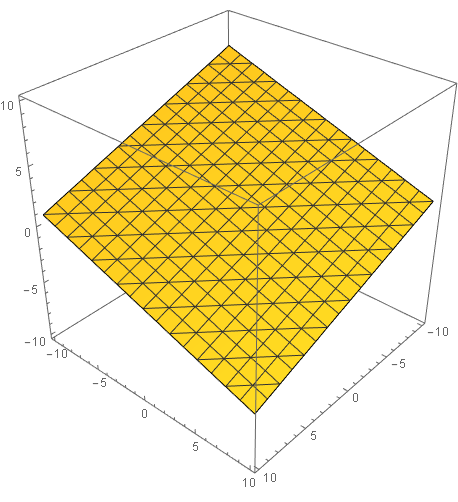
\includegraphics[scale=0.45]{pages/images/plane.png}
		\caption{Example of a plane}	
		\label{fig:test_figure}
	\end{center}
\end{figure}
%-------------------------------------------------------------------------%


\subsubsection{Scaler Equation of a Plane}
Given that $\vv{n} = \langle N_x, N_y, N_z \rangle$, we can compute the dot product to get the scaler equation of the plane. Let $\vv{r}$ = $\langle x,y,z \rangle$ and $\vv{r_o} = \langle x_o,y_o,z_o \rangle$.

\begin{align*}
	\vv{n} \cdot (\vv{r} - \vv{r_o}) &= 0 \\ 
	\vv{n} \cdot \langle x-x_o,y-y_o, z-z_o  \rangle &= 0 \\ 
	(x-x_o)N_x + (y-y_o)N_y + (z-z_o)N_z &= 0 
\end{align*}

Note that if we expanded the scaler equations out and set the equation to a different value, the coefficients of the terms will give the normal vector as well. 

\subsubsection{Angle Between Planes}
Given two planes $L_1$ $L_2$, we can figure out the angle between these two planes by considering their normal vectors. Given 
$\vv{L_{(1)n}}$ and $\vv{L_{(2)n}}$, consider their dota product. 

\begin{equation*}
\vv{L_{(1)n}} \cdot \vv{L_{(2)n}} = |L_{(1)n}|L_{(2)n}|\cos(\theta)
\end{equation*}

We can solve for the $\cos(\theta)$, 

\begin{equation*}
	\frac{\vv{L_{(1)n}} \cdot \vv{L_{(2)n}}}{|L_{(1)n}|L_{(2)n}|} = \cos(\theta)
\end{equation*}

Don't forget that inverse cosine has a specific domain.

\subsubsection{Examples}
Given $P(1,3,2)$ and $Q(3,-1,6)$ and $R(5,2,0)$, find the plane described by these points. First we need vectors on that said plane. So we will use $\vv{QP}$ and $\vv{QR}$. 

\begin{align*}
	\vv{QP} &= \langle -2,4,4 \rangle  \\ 
	\vv{QR} &= \langle 2,3,-6 \rangle 
\end{align*}

We know that the cross between those two vectors will give us the normal vector of the plane. 

\begin{equation*}
	\vv{n} = \vv{QP} \times \vv{QR} = \begin{vmatrix}
		i & j & k \\ 
		-2 & 4 & 4 \\  
		2 &3 & -6  \\ 
	\end{vmatrix} \begin{matrix}
		i & j \\ 
		-2 & 4 \\ 
		2 & 3 \\ 
	\end{matrix}
\end{equation*}

The cross product gives us a normal vector.
\begin{equation*}
	\vv{n} = \langle -36,-4,-14 \rangle 
\end{equation*}

Using the vector equation of a plane, using any of the initial given points.

\begin{equation*}
	\vv{n} \cdot (\vv{r}-\vv{P}) = 0
\end{equation*}
Expanding it out and computing the dot product will give us the scaler equation of a plane 
\begin{equation*}
	-36(x-1)-4(y-3)-14(z-2)=0
\end{equation*}
\subsubsection{Intersecting Planes}
Lets say we are given two planes that intersect each other. 
%-------------------------------------------------------------------------%
\begin{figure}[H]
	\begin{center}
		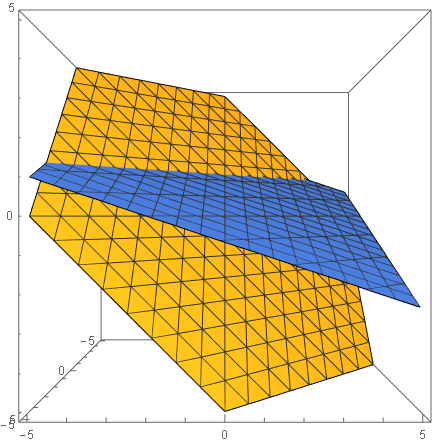
\includegraphics[scale=0.45]{pages/images/plane_intersection.png}
		\caption{Two planes intersecting}	
		\label{fig:test_figure}
	\end{center}
\end{figure}
%-------------------------------------------------------------------------%
To determine the equation of the intersecting line we are going to need a point and a vector point in the direction of that said line. The point is the harder part. Consider the scaler equations of the planes, 

\begin{equation*}
	ax + by + cz = k 
\end{equation*}

Since the domain of this equation is all $\mathbb{R}$, we can set on of these variables to any number we want. If we set $x=0$ for both equations of planes we can get a system of equations for two terms. Let's say we found this point, $P(x_o,y_o,z_o)$, we still need a vector. Since we know that the normal vectors are perpendicular to the planes they describe, the cross product between those two normal vectors will yield intersection vector. 

\begin{equation*}
	\vv{v} = \vv{L_1} \times \vv{L_2}
\end{equation*}
\begin{equation*}
	\vv{I_f} = \vv{OP} + \vv{v}t 
\end{equation*}